% Figure 1 -- architecture of redcap2hdcat. Black-and-white line art.
% Build: make -C paper figures   (PDF for the review copy; EPS and 1,200 dpi TIFF to submit)
\documentclass[border=2pt]{standalone}
\usepackage[T1]{fontenc}
\usepackage[scaled=0.92]{helvet}
\renewcommand{\familydefault}{\sfdefault}
\usepackage{tikz}
\usetikzlibrary{positioning,arrows.meta,fit,calc}
\begin{document}
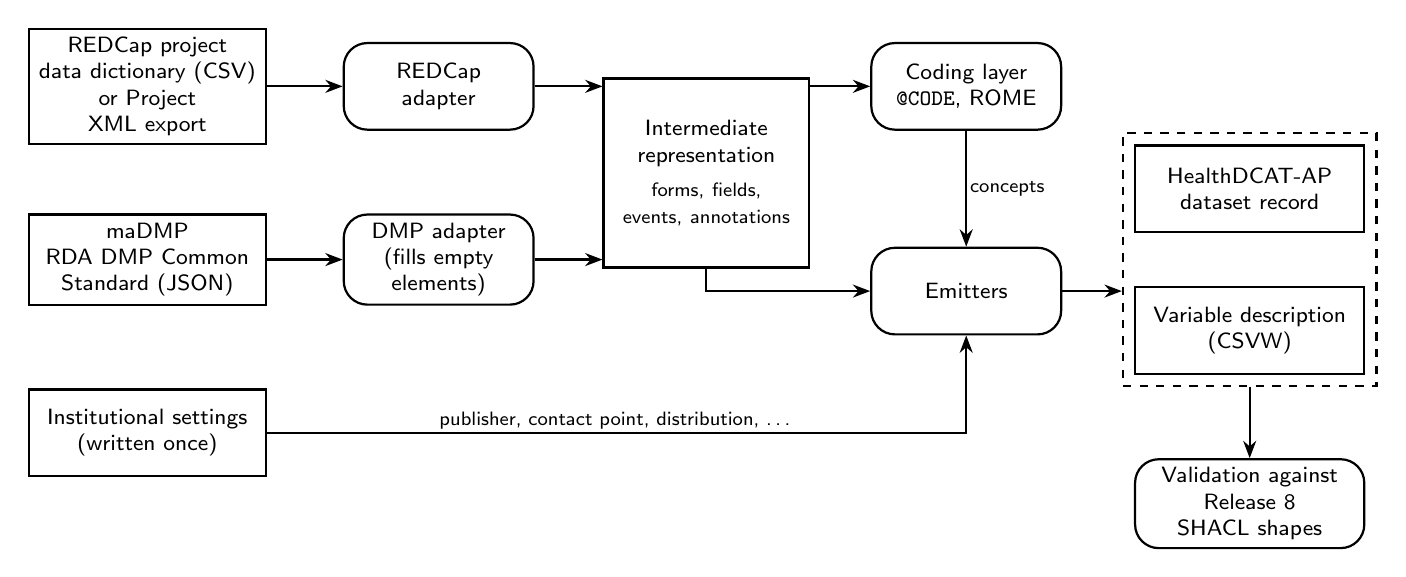
\begin{tikzpicture}[
  font=\footnotesize,
  >={Stealth[length=2.2mm]},
  data/.style={draw, thick, align=center, minimum height=11mm, inner sep=3pt},
  proc/.style={draw, thick, rounded corners=3mm, align=center, minimum height=11mm, inner sep=3pt},
  arr/.style={->, thick},
  lab/.style={font=\scriptsize, align=center, fill=white, inner sep=1pt},
]
% inputs
\node[data, text width=28mm] (redcap) at (0,  2.2) {REDCap project\\data dictionary (CSV)\\or Project XML export};
\node[data, text width=28mm] (dmp)    at (0,  0.0) {maDMP\\RDA DMP Common\\Standard (JSON)};
\node[data, text width=28mm] (cfg)    at (0, -2.2) {Institutional settings\\(written once)};
% adapters
\node[proc, text width=22mm] (ra) at (3.7, 2.2) {REDCap\\adapter};
\node[proc, text width=22mm] (da) at (3.7, 0.0) {DMP adapter\\(fills empty\\elements)};
% intermediate representation
\node[data, text width=24mm, minimum height=24mm] (ir) at (7.1, 1.1)
  {Intermediate\\representation\\[3pt]{\scriptsize forms, fields,}\\{\scriptsize events, annotations}};
% coding and emitters
\node[proc, text width=22mm] (code) at (10.4, 2.2) {Coding layer\\\texttt{@CODE}, ROME};
\node[proc, text width=22mm] (emit) at (10.4, -0.4) {Emitters};
% outputs
\node[data, text width=27mm] (rec)  at (14.0, 0.9) {HealthDCAT-AP\\dataset record};
\node[data, text width=27mm] (var)  at (14.0, -0.9) {Variable description\\(CSVW)};
\node[draw, thick, dashed, inner sep=4pt, fit=(rec)(var)] (out) {};
\node[proc, text width=27mm] (val) at (14.0, -3.1) {Validation against\\Release~8 SHACL shapes};
% flows
\draw[arr] (redcap) -- (ra);
\draw[arr] (dmp) -- (da);
\draw[arr] (ra.east) -- (ra.east -| ir.west);
\draw[arr] (da.east) -- (da.east -| ir.west);
\draw[arr] (ir.east |- code.west) -- (code.west);
\draw[arr] (code) -- node[lab, right]{concepts} (emit);
\draw[arr] (ir.south) |- (emit.west);
\draw[arr] (cfg.east) -| node[lab, pos=0.25, above]{publisher, contact point, distribution, \dots} (emit.south);
\draw[arr] (emit.east) -- (emit.east -| out.west);
\draw[arr] (out.south) -- (val.north);
\end{tikzpicture}
\end{document}
